\chapter{SoC与系统移植}\label{chap:07-soc-and-system}

\section{芯片整体SoC设计}\label{sec:07-soc-and-system-001}

MegaSoC 是由北航百芯计划团队开发的一款 SoC 框架，支持使用 AXI 总线的 LoongArch 指令集处理器的正常工作。

\subsection{OpenMegaSoC简介}\label{sec:07-soc-and-system-002}

\begin{enumerate}
\def\labelenumi{\arabic{enumi}.}
\tightlist
\item
  支持外设
\end{enumerate}

OpenMegaSoC 提供了 SPI、SDIO、I2S、VGA、Ethernet、UART、CDBUS、I2C 等硬件外设支持。

\begin{figure}
\centering
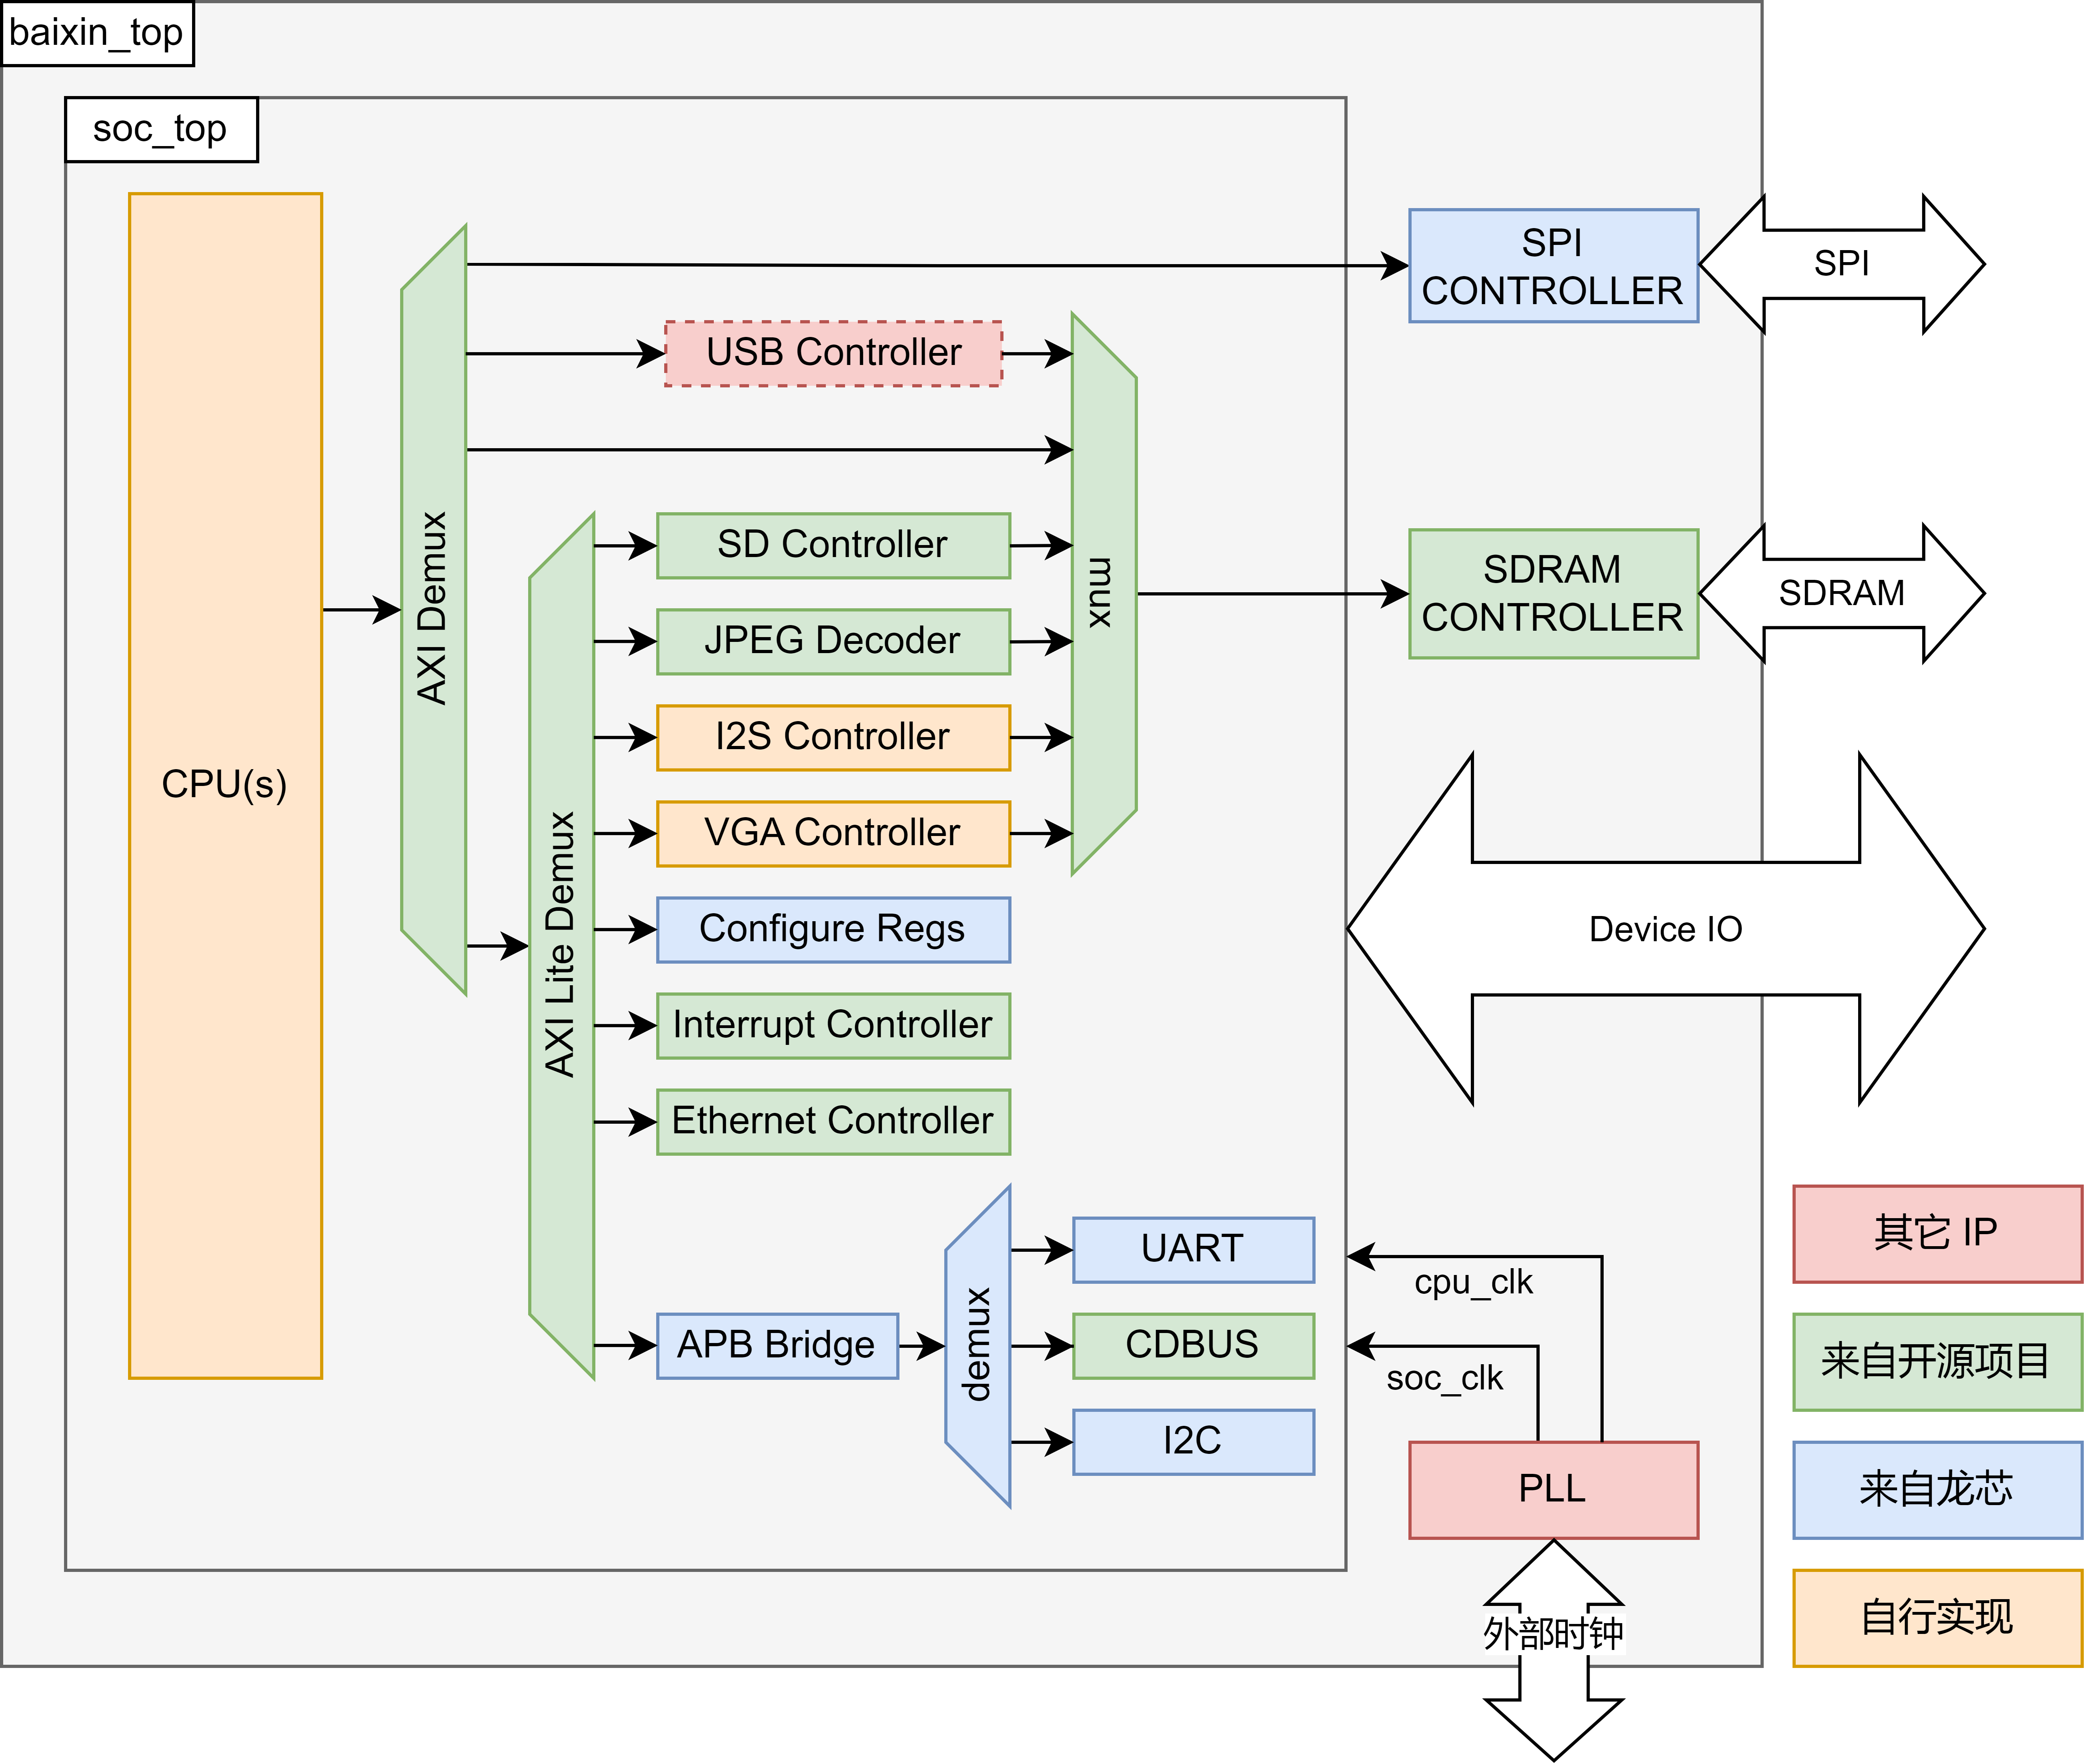
\includegraphics[width=\linewidth]{assets/07/megasoc.drawio.png}
\caption{百芯部署整体框架图}\label{fig:07-megasoc}
\end{figure}

\begin{enumerate}
\def\labelenumi{\arabic{enumi}.}
\setcounter{enumi}{1}
\tightlist
\item
  AXI4 外设地址映射
\end{enumerate}

\begin{longtable}[]{@{}
  >{\raggedright\arraybackslash}p{(\linewidth - 4\tabcolsep) * \real{0.6022}}
  >{\raggedright\arraybackslash}p{(\linewidth - 4\tabcolsep) * \real{0.2688}}
  >{\raggedright\arraybackslash}p{(\linewidth - 4\tabcolsep) * \real{0.1290}}@{}}
\toprule\noalign{}
\begin{minipage}[b]{\linewidth}\raggedright
Address Range
\end{minipage} & \begin{minipage}[b]{\linewidth}\raggedright
Device
\end{minipage} & \begin{minipage}[b]{\linewidth}\raggedright
Select Value
\end{minipage} \\
\midrule\noalign{}
\endhead
\bottomrule\noalign{}
\endlastfoot
\texttt{0x00000000\ -\ 0x0FFFFFFF} & Memory Controller & 0 \\
\texttt{0x1C000000\ -\ 0x1C0FFFFF}\newline{}\texttt{0x1D000000\ -\ 0x1D00FFFF} & SPI Device & 1 \\
\texttt{0x1D010000\ -\ 0x1D0FFFFF} & AXI-Lite Device & 2 \\
\texttt{0x1D100000\ -\ 0x1D1FFFFF} & USB Controller & 3 \\
Other Addresses & AXI-Lite Device (Default) & 2 \\
\end{longtable}

\begin{enumerate}
\def\labelenumi{\arabic{enumi}.}
\setcounter{enumi}{2}
\tightlist
\item
  AXI4 Lite 外设地址映射
\end{enumerate}

\begin{longtable}[]{@{}
  >{\raggedright\arraybackslash}p{(\linewidth - 4\tabcolsep) * \real{0.3731}}
  >{\raggedright\arraybackslash}p{(\linewidth - 4\tabcolsep) * \real{0.4478}}
  >{\raggedright\arraybackslash}p{(\linewidth - 4\tabcolsep) * \real{0.1791}}@{}}
\toprule\noalign{}
\begin{minipage}[b]{\linewidth}\raggedright
Address Range
\end{minipage} & \begin{minipage}[b]{\linewidth}\raggedright
Device
\end{minipage} & \begin{minipage}[b]{\linewidth}\raggedright
Select Value
\end{minipage} \\
\midrule\noalign{}
\endhead
\bottomrule\noalign{}
\endlastfoot
\texttt{0x1D010000\ -\ 0x1D03FFFF} & APB Devices (UART, I2C, CDBUS) & 1 \\
\texttt{0x1D040000\ -\ 0x1D04FFFF} & Configuration Registers & 2 \\
\texttt{0x1D050000\ -\ 0x1D05FFFF} & Ethernet Controller & 3 \\
\texttt{0x1D060000\ -\ 0x1D06FFFF} & Interrupt Controller & 4 \\
\texttt{0x1D070000\ -\ 0x1D07FFFF} & SD Controller & 5 \\
\texttt{0x1D0A0000\ -\ 0x1D0AFFFF} & JPEG Controller & 6 \\
\texttt{0x1D0B0000\ -\ 0x1D0BFFFF} & I2S Controller-0（DMA） & 7 \\
\texttt{0x1D0C0000\ -\ 0x1D0CFFFF} & I2S Controller-1（GEN） & 8 \\
\texttt{0x1D0D0000\ -\ 0x1D0DFFFF} & VGA Controller & 9 \\
Other Addresses & SRAM Controller (Default) & 0 \\
\end{longtable}

\begin{enumerate}
\def\labelenumi{\arabic{enumi}.}
\setcounter{enumi}{3}
\tightlist
\item
  IP 来源
\end{enumerate}

\begin{longtable}[]{@{}
  >{\raggedright\arraybackslash}p{(\linewidth - 4\tabcolsep) * \real{0.2016}}
  >{\raggedright\arraybackslash}p{(\linewidth - 4\tabcolsep) * \real{0.4651}}
  >{\raggedright\arraybackslash}p{(\linewidth - 4\tabcolsep) * \real{0.3333}}@{}}
\toprule\noalign{}
\begin{minipage}[b]{\linewidth}\raggedright
名称
\end{minipage} & \begin{minipage}[b]{\linewidth}\raggedright
来源
\end{minipage} & \begin{minipage}[b]{\linewidth}\raggedright
作用
\end{minipage} \\
\midrule\noalign{}
\endhead
\bottomrule\noalign{}
\endlastfoot
loongson-blocks & \url{https://gitee.com/loongson-edu/chiplab/tree/chiplab_diff/IP} & 提供UART、CONFREG、SPI控制器 \\
pulp-axi & \url{https://github.com/pulp-platform/axi} & 用于高性能片上通信的 AXI SystemVerilog 模块 \\
pulp-common\_cells & \url{https://github.com/pulp-platform/common_cells} & 常用模块、头文件 \\
register\_interface & \url{https://github.com/pulp-platform/register_interface} & 通用寄存器接口 \\
ultraembedded-jpeg\_decoder & \url{https://github.com/ultraembedded/core_jpeg_decoder} & JPEG解码器 \\
Xilinx-AXI-Intc & Xilinx开源IP & 中断控制器 \\
Xilinx-emaclite & Xilinx开源IP & 以太网控制器 \\
Xilinx-primitive & Xilinx开源IP & cdc、fifo \\
Xilinx-AXIAHB & Xilinx开源IP & AXI-AHB总线桥 \\
ZipCPU-wb2axip & \url{https://github.com/ZipCPU/wb2axip} & 总线互连、桥接器和其他组件 \\
i2c-slave & \url{https://github.com/freecores/i2cslave} & I2C从设备 \\
opencores-i2c & \url{https://github.com/fabriziotappero/ip-cores/tree/communication_controller_i2c_controller_core\#vhdlverilog-ip-cores-repository} & I2C主设备 \\
axi\_to\_i2s & 自主设计 & AXI控制的I2S输出模块 \\
axi-hdmi & 自主设计 & SII-146芯片控制器 \\
dukelec-cdbus\_ip & \url{https://github.com/dukelec/cdbus} & CDBUS控制器 \\
axi-sdc & \url{https://github.com/mczerski/SD-card-controller} & SD卡控制器 \\
\end{longtable}

\begin{enumerate}
\def\labelenumi{\arabic{enumi}.}
\setcounter{enumi}{4}
\tightlist
\item
  支持平台
\end{enumerate}

OpenMegaSoC 尽可能以 RTL 形式提供使用到的所有模块，因此对硬件开发平台有最小化的要求。

目前本项目提供面向龙芯百芯计划开发板（7A200T）、北航百芯计划开发板（7K325T）、ZU15MINI开发板（XCZU15EG）三款 FPGA 开发板的支持。

本项目最小化了对厂商相关的 Primitive 使用。对于不同的开发平台，只需要准备 SRAM 、PLL 这两类模块既可。

你可以很轻松的将本项目 SoC 部署到其它平台。具体可参考 Menufacturer/Xilinx 目录下的实现，完成约束和 SRAM 模块的替换即可。

\begin{enumerate}
\def\labelenumi{\arabic{enumi}.}
\setcounter{enumi}{5}
\tightlist
\item
  视频接口说明
\end{enumerate}

OpenMegaSoC 对外输出 RGB888 全彩视频，但需要借助 SII-164 芯片辅助。具体输出格式，请参考 SII-164 芯片数据手册。

视频中的 24 位色彩信号采用双边沿时钟采样格式并行传输。SoC 内部按照 VGA 时序生成视频信号，并对 RGB 数据信号做双边沿采样操作。

也可以修改 SoC 中的相关数据通路，改为直接输出单边沿采样的 VGA 信号。

\begin{enumerate}
\def\labelenumi{\arabic{enumi}.}
\setcounter{enumi}{6}
\tightlist
\item
  音频接口说明
\end{enumerate}

OpenMegaSoC 对外输出 I2S 格式的音频，需要外部 DAC 配合完成模拟音频信号的输出。同时建议采用来自外部晶振的音频时钟以获得较好的音频质量（也可由内部 PLL 产生）。

对于龙芯提供的两款开发板，均需要使用拓展 IO 完成对 I2S 音频输出的支持。

\begin{enumerate}
\def\labelenumi{\arabic{enumi}.}
\setcounter{enumi}{7}
\tightlist
\item
  目录结构
\end{enumerate}

\begin{itemize}
\tightlist
\item
  Board 文件夹 存放板级相关文件，包括板级顶层、板级 FPGA IO 约束、开发板工程。
\item
  General 文件夹 存放平台无关代码，包括 SoC 顶层（soc\_top）、SoC 使用到的 IP 核等。若需要修改核心地址映射，或者添加新的外设设备，需要对这一层进行修改
\item
  Manufacture 存放平台相关代码，目前仅有 Xilinx 平台下的相关代码支持。用户需要在这里提供本项目使用的不同规格 SRAM。 本项目使用双口及单口 SRAM，具体涉及的 SRAM 规格及模块名称，可参考 \texttt{Xilinx/dpram\_wrapper.sv} 及 \texttt{Xilinx/spram\_wrapper.sv} 文件。
\end{itemize}

\subsection{SoC适配}\label{sec:07-soc-and-system-003}

MegaSoC总体采用AXI4接口进行片内互联，CPU相关可参考\texttt{MegaSoC/General/SoC/cpu\_wrapper.sv}文件，其中包含了CPU的实例化：

% 代码语言：BookVerilog
\begin{CodeBlock}[language=BookVerilog]
// cpu
`ifdef EULA_CORE
  assign cpu_arlen[`Larlen - 1 : 4] = 0;
  assign cpu_awlen[`Lawlen - 1 : 4] = 0;
`endif
mycpu_mega_top cpu_mid (
  .aclk         (cpu_clk),
  .ext_int      ({2'b0, int_cpu}),  //232 only 5bit
  .aresetn      (cpu_aresetn    ),
  .global_reset (cpu_global_reset),
 
  .arid         (cpu_arid[3:0] ),
  .araddr       (cpu_araddr    ),
`ifdef EULA_CORE
  .arlen        (cpu_arlen[3:0]),
`else
  .arlen        (cpu_arlen     ),
`endif
  .arsize       (cpu_arsize    ),
  .arburst      (cpu_arburst   ),
  .arlock       (cpu_arlock    ),
  .arcache      (cpu_arcache   ),
  .arprot       (cpu_arprot    ),
  .arvalid      (cpu_arvalid   ),
  .arready      (cpu_arready   ),
  .rid          (cpu_rid[3:0]  ),
  .rdata        (cpu_rdata     ),
  .rresp        (cpu_rresp     ),
  .rlast        (cpu_rlast     ),
  .rvalid       (cpu_rvalid    ),
  .rready       (cpu_rready    ),
  .awid         (cpu_awid[3:0] ),
  .awaddr       (cpu_awaddr    ),
`ifdef EULA_CORE
  .awlen        (cpu_awlen[3:0]),
`else
  .awlen        (cpu_awlen     ),
`endif
  .awsize       (cpu_awsize    ),
  .awburst      (cpu_awburst   ),
  .awlock       (cpu_awlock    ),
  .awcache      (cpu_awcache   ),
  .awprot       (cpu_awprot    ),
  .awvalid      (cpu_awvalid   ),
  .awready      (cpu_awready   ),
  .wdata        (cpu_wdata     ),
  .wstrb        (cpu_wstrb     ),
  .wlast        (cpu_wlast     ),
  .wvalid       (cpu_wvalid    ),
  .wready       (cpu_wready    ),
  .bid          (cpu_bid[3:0]  ),
  .bresp        (cpu_bresp     ),
  .bvalid       (cpu_bvalid    ),
  .bready       (cpu_bready    ),

  .debug_wb_pc  (debug_wb_pc   ),
  .debug_wb_instr(debug_wb_instr),
  .debug_wb_rf_wdata(debug_wb_rf_wdata)
);
\end{CodeBlock}

然后在CPU顶层封装\texttt{cpu\_wrapper}模块，规范化其对外接口，使得SoC整体较为容易管理所有Master和Slave设备。

\section{Linux 系统板级移植}\label{sec:07-soc-and-system-004}

\subsection{Linux 设备树介绍}\label{sec:07-soc-and-system-005}

设备树（Device Tree）是一种描述硬件结构和设备信息的数据结构，用于在嵌入式系统中动态配置硬件设备和驱动程序。设备树文件通常使用.dts或.dtsi后缀，是一种描述硬件平台和设备的中间编译形式，最终会被编译成.dtb文件，供操作系统内核使用。

设备树文件（.dts/.dtsi）中包含以下几类基本对象：

\begin{enumerate}
\def\labelenumi{\arabic{enumi}.}
\tightlist
\item
  节点（Node）：
\end{enumerate}

\begin{itemize}
\item
  设备树中的基本单位是节点，用来描述硬件设备或者硬件资源。每个节点由一个标签（label）和一组属性（properties）组成。
\item
  标签通常是设备的名称或者类型，例如 ``uart''、``ethernet''。
\item
  属性（properties）则是描述设备特性和配置信息的键值对，例如中断号、内存地址等。
\end{itemize}

\begin{enumerate}
\def\labelenumi{\arabic{enumi}.}
\setcounter{enumi}{1}
\tightlist
\item
  属性（Properties）：
\end{enumerate}

\begin{itemize}
\item
  每个设备树节点可以有多个属性，用来描述节点所表示的硬件设备的详细信息。
\item
  属性包括必选属性（required properties）和可选属性（optional properties），必选属性是设备驱动程序所必需的，而可选属性则是可选的配置参数。
\end{itemize}

\begin{enumerate}
\def\labelenumi{\arabic{enumi}.}
\setcounter{enumi}{2}
\tightlist
\item
  绑定（Binding）：
\end{enumerate}

\begin{itemize}
\item
  绑定是设备树文件中的一种约定，用于将设备树节点和设备驱动程序关联起来。
\item
  绑定通过设备树节点的标签和设备驱动程序的名称或类型来实现，从而告知内核如何将设备树中的设备节点与相应的驱动程序匹配。
\end{itemize}

\begin{enumerate}
\def\labelenumi{\arabic{enumi}.}
\setcounter{enumi}{3}
\tightlist
\item
  片段（Fragment）：
\end{enumerate}

\begin{itemize}
\item
  设备树片段是.dtsi文件中的一个部分，通常用于包含设备树的一部分配置信息。它们可以被其他设备树文件（包括主设备树文件）包含和重用。
\item
  设备树片段有助于组织和管理设备树的复杂性，尤其是在大型项目或者多个硬件平台中。
\end{itemize}

\begin{enumerate}
\def\labelenumi{\arabic{enumi}.}
\setcounter{enumi}{4}
\tightlist
\item
  包含（Include）：
\end{enumerate}

\begin{itemize}
\tightlist
\item
  设备树文件可以使用包含（include）指令来引入其他设备树文件或者设备树片段（.dtsi文件），以便在当前设备树文件中重用已定义的节点和属性。
\end{itemize}

通过上述基本对象，设备树文件能够有效地描述和配置嵌入式系统中的硬件设备，使得Linux内核能够动态识别和管理这些设备，实现设备驱动程序的加载和运行。

以下将以MegaSoC为例，介绍如何在Linux中添加相应的设备树支持。

首先在\texttt{linux/arch/loongarch/boot/dts/loongson}文件夹添加\texttt{la32rmega\_demo.dts}文件：

% 代码语言：BookDTS
\begin{CodeBlock}[language=BookDTS]
/dts-v1/;
/{
    model = "loongson,generic";
    compatible = "loongson,loongson3";
    #address-cells = <1>;
    #size-cells = <1>;

    aliases {
        serial0 = &cpu_uart0;
        mmc0 = &mmc0;
    };

    chosen {
        stdout-path = "serial0:230400n8";
        bootargs = "earlycon";
        ranges;
        framebuffer: framebuffer@7800000 {
            compatible = "simple-framebuffer";
            reg = <0xf000000 (800 * 600 * 2 * 4)>;
            width = <800>;
            height = <600>;
            stride = <(800 * 2)>;
            format = "r5g6b5";
        }; 
    };

	socclk: socclk {
		compatible = "fixed-clock";
		clock-frequency = <133333333>;
		#clock-cells = <0>;
	};

	i2sclk: i2sclk {
		compatible = "fixed-clock";
		clock-frequency = <24576000>;
		#clock-cells = <0>;
	};

    memory {
        name = "memory";
        device_type = "memory";
        reg =  <0x00000000  0x0f000000>;
    };

	cpuic: interrupt-controller {
	    compatible = "loongson,cpu-interrupt-controller";
        interrupt-controller;
		#interrupt-cells = <1>;
	};

	soc {
		compatible = "simple-bus";
		#address-cells = <1>;
		#size-cells = <1>;
		ranges = <0x10000000 0x10000000 0x10000000>;

        axi_intc_0: interrupt-controller@1d060000 {
                #interrupt-cells = <1>;
                compatible = "xlnx,xps-intc-1.00.a";
                interrupt-controller;
                interrupt-parent = <&cpuic>;
                interrupts = <1>;
                reg = <0x1d060000 0x1000>;
                xlnx,kind-of-intr = <0x1>;
                xlnx,num-intr-inputs = <0x8>;
        };

        cpu_uart0: serial@0x1d010000 {
		    device_type = "serial";
		    compatible = "ns16550a";
		    reg = <0x1d010000 0x1000>;
            clock-frequency = <133333333>;
		    reg-offset = <0x0000>;
		    reg-io-width = <1>;
		    reg-shift = <0>;
		    current-speed = <230400>;
            interrupt-parent = <&cpuic>;
		    interrupts = <5>;
        };

        i2c1: i2c@1d020000 {
            compatible = "opencores,i2c-ocores";
            reg = <0x1d020000 0x1000>;
            interrupt-parent = <&axi_intc_0>;
            interrupts = <4>;
            clocks = <&socclk>;
            clock-frequency = <400000>;
            reg-shift = <0>;	/* 8 bit registers */
            reg-io-width = <1>;	/* 8 bit read/write */
        };

        axi_ethernetlite: ethernet@1d050000 {
			compatible = "xlnx,xps-ethernetlite-3.00.a";
			device_type = "network";
			mac-address = [19 98 00 01 00 29];
			phy-handle = <&phy0>;
			reg = <0x1d050000 0x10000>;
			xlnx,duplex = <0x1>;
			xlnx,include-global-buffers = <0x1>;
			xlnx,include-internal-loopback = <0x0>;
			xlnx,include-mdio = <0x1>;
			xlnx,instance = "axi_ethernetlite_inst";
			xlnx,rx-ping-pong = <0x1>;
			xlnx,s-axi-id-width = <0x1>;
			xlnx,tx-ping-pong = <0x1>;
			xlnx,use-internal = <0x0>;
			interrupt-parent = <&axi_intc_0>;
			interrupts = <0>;
			mdio {
				#address-cells = <1>;
				#size-cells = <0>;
				phy0: phy@1 {
					device_type = "ethernet-phy";
					reg = <1>;
				} ;
			} ;
		} ;

        mmc0: mmc@1d070000 {
			compatible = "riscv,axi-sd-card-1.0";
			clock = <100000000>;
			reg = <0x1d070000 0x64>;
			fifo-depth = <256>;
			bus-width = <4>;
			max-frequency = <25000000>;
            interrupt-parent = <&cpuic>;
			interrupts = <6>;
            cap-sd-highspeed;
            cap-mmc-highspeed;
            cap-mmc-hw-reset;
            no-sdio;
		};

		usbphy: usbphy {
			#phy-cells = <0>;
			compatible = "usb-nop-xceiv";
			status = "okay";
		};
		usb: usb@1d100000 {
			compatible = "snps,dwc2";
			reg = <0x1d100000 0x40000>;
			interrupt-parent = <&axi_intc_0>;
			interrupts = <2>;
            clocks = <&socclk>;
			clock-names = "otg";
            phys = <&usbphy>;
            phy-names = "usb2-phy";
            dr_mode = "otg";
			status = "okay";
		};

        audio_ss_0_audio_formatter_0: audio_formatter@1d0b0000 {
            compatible = "xlnx,audio-formatter-1.0";
            interrupt-names = "irq_mm2s";
            interrupt-parent = <&cpuic>;
            interrupts = <3>;
            reg = <0x1d0b0000 0x1000>;
            xlnx,tx = <&i2s_transmitter_0>;
            // xlnx,rx = <&i2s_receiver>;
            clock-names = "s_axi_lite_aclk", "m_axis_mm2s_aclk", "aud_mclk";
            clocks = <&socclk>, <&socclk>, <&i2sclk>;
        };

        i2s_transmitter_0: i2s_transmitter@1d0c0000 {
            compatible = "xlnx,i2s-transmitter-1.0";
            clock-names = "s_axi_ctrl_aclk", "aud_mclk", "s_axis_aud_aclk";
            clocks = <&socclk>, <&i2sclk>, <&socclk>;
            reg = <0x1d0c0000 0x10000>;
            xlnx,dwidth = <0x10>;
            xlnx,num-channels = <1>;
            xlnx,snd-pcm = <&audio_ss_0_audio_formatter_0>;
        };
    };
};
\end{CodeBlock}

可以看到，我们在设备树中添加了时钟、存储器、串口、中断控制器、以太网、MMC等设备，并编写了对应属性，然后，在\texttt{linux/arch/boot/dts/loongson/Makefile}中添加：

% 代码语言：BookMake
\begin{CodeBlock}[language=BookMake]
dtb-$(CONFIG_LS_SOC) += loongson32_ls.dtb
dtb-$(CONFIG_BX_SOC) += loongson32_bx.dtb
dtb-$(CONFIG_MEGA_SOC_FPGA) += la32rmega_demo.dtb # 新增
\end{CodeBlock}

之后，添加\texttt{linux/arch/loongarch/configs/la32rmega\_defconfig}文件：

% 代码语言：BookConfig
\begin{CodeBlock}[language=BookConfig]
CONFIG_SYSVIPC=y
CONFIG_NO_HZ=y
CONFIG_HIGH_RES_TIMERS=y
CONFIG_BPF_SYSCALL=y
CONFIG_PREEMPT=y
CONFIG_BSD_PROCESS_ACCT=y
CONFIG_BSD_PROCESS_ACCT_V3=y
CONFIG_LOG_BUF_SHIFT=18
CONFIG_MEMCG=y
CONFIG_CFS_BANDWIDTH=y
CONFIG_RT_GROUP_SCHED=y
CONFIG_CGROUP_PIDS=y
CONFIG_CGROUP_FREEZER=y
CONFIG_CGROUP_DEVICE=y
CONFIG_CGROUP_CPUACCT=y
CONFIG_CGROUP_PERF=y
CONFIG_CGROUP_BPF=y
CONFIG_CHECKPOINT_RESTORE=y
CONFIG_SCHED_AUTOGROUP=y
CONFIG_SYSFS_DEPRECATED=y
CONFIG_RELAY=y
CONFIG_EXPERT=y
CONFIG_USERFAULTFD=y
CONFIG_PERF_EVENTS=y
# CONFIG_VM_EVENT_COUNTERS is not set
# CONFIG_SLUB_DEBUG is not set
# CONFIG_COMPAT_BRK is not set
CONFIG_MACH_LOONGSON_32=y
CONFIG_FORCE_MAX_ZONEORDER=12
# CONFIG_DMI is not set
CONFIG_EFI=y
# CONFIG_SECCOMP is not set
CONFIG_ARCH_MMAP_RND_BITS=12
CONFIG_BINFMT_MISC=y
CONFIG_NET=y
CONFIG_UNIX=y
CONFIG_INET=y
CONFIG_IP_MULTICAST=y
CONFIG_PCCARD=y
CONFIG_UEVENT_HELPER=y
CONFIG_DEVTMPFS=y
CONFIG_DEVTMPFS_MOUNT=y
CONFIG_MTD=y
CONFIG_MTD_CMDLINE_PARTS=y
CONFIG_MTD_PARTITIONED_MASTER=y
CONFIG_MTD_CFI=y
CONFIG_MTD_JEDECPROBE=y
CONFIG_MTD_CFI_INTELEXT=y
CONFIG_MTD_CFI_AMDSTD=y
CONFIG_MTD_CFI_STAA=y
CONFIG_MTD_RAM=y
CONFIG_MTD_ROM=y
CONFIG_MTD_RAW_NAND=y
CONFIG_MTD_NAND_LS1A=y
# CONFIG_MTD_NAND_ECC_SW_HAMMING is not set
CONFIG_MTD_NAND_ECC_SW_BCH=y
CONFIG_OF=y
CONFIG_OF_OVERLAY=y
CONFIG_SCSI=y
CONFIG_BLK_DEV_SD=y
CONFIG_NETDEVICES=y
CONFIG_STMMAC_ETH=y
CONFIG_XILINX_EMACLITE=y
CONFIG_DMFE_MAC=y
CONFIG_INPUT_MOUSEDEV=y
CONFIG_INPUT_MOUSEDEV_PSAUX=y
CONFIG_KEYBOARD_XTKBD=y
CONFIG_MOUSE_PS2_ELANTECH=y
CONFIG_MOUSE_PS2_SENTELIC=y
CONFIG_MOUSE_SERIAL=y
CONFIG_INPUT_JOYSTICK=y
CONFIG_JOYSTICK_ANALOG=y
CONFIG_JOYSTICK_A3D=y
CONFIG_JOYSTICK_ADI=y
CONFIG_JOYSTICK_COBRA=y
CONFIG_JOYSTICK_GF2K=y
CONFIG_JOYSTICK_GRIP=y
CONFIG_JOYSTICK_GRIP_MP=y
CONFIG_JOYSTICK_GUILLEMOT=y
CONFIG_JOYSTICK_INTERACT=y
CONFIG_JOYSTICK_SIDEWINDER=y
CONFIG_JOYSTICK_TMDC=y
CONFIG_JOYSTICK_IFORCE=y
CONFIG_JOYSTICK_IFORCE_USB=y
CONFIG_JOYSTICK_IFORCE_232=y
CONFIG_JOYSTICK_WARRIOR=y
CONFIG_JOYSTICK_MAGELLAN=y
CONFIG_JOYSTICK_SPACEORB=y
CONFIG_JOYSTICK_SPACEBALL=y
CONFIG_JOYSTICK_STINGER=y
CONFIG_JOYSTICK_TWIDJOY=y
CONFIG_JOYSTICK_ZHENHUA=y
CONFIG_JOYSTICK_AS5011=y
CONFIG_JOYSTICK_JOYDUMP=y
CONFIG_JOYSTICK_XPAD=y
CONFIG_JOYSTICK_XPAD_FF=y
CONFIG_JOYSTICK_XPAD_LEDS=y
CONFIG_JOYSTICK_PXRC=y
CONFIG_JOYSTICK_QWIIC=y
CONFIG_JOYSTICK_FSIA6B=y
CONFIG_INPUT_MISC=y
CONFIG_SERIO_RAW=y
CONFIG_LEGACY_PTY_COUNT=16
CONFIG_SERIAL_8250=y
CONFIG_SERIAL_8250_CONSOLE=y
CONFIG_SERIAL_8250_NR_UARTS=16
CONFIG_SERIAL_8250_RUNTIME_UARTS=16
CONFIG_SERIAL_8250_EXTENDED=y
CONFIG_SERIAL_8250_MANY_PORTS=y
CONFIG_SERIAL_8250_SHARE_IRQ=y
CONFIG_SERIAL_8250_RSA=y
CONFIG_SERIAL_OF_PLATFORM=y
CONFIG_SERIAL_NONSTANDARD=y
CONFIG_IPMI_HANDLER=y
CONFIG_IPMI_DEVICE_INTERFACE=y
CONFIG_IPMI_SI=y
CONFIG_I2C=y
CONFIG_I2C_CHARDEV=y
# CONFIG_I2C_HELPER_AUTO is not set
CONFIG_I2C_OCORES=y
CONFIG_PPS=y
# CONFIG_PTP_1588_CLOCK is not set
CONFIG_GPIOLIB=y
CONFIG_GPIO_SYSFS=y
CONFIG_RC_CORE=y
CONFIG_LIRC=y
CONFIG_RC_DECODERS=y
CONFIG_IR_MCE_KBD_DECODER=y
CONFIG_FB=y
CONFIG_FB_FOREIGN_ENDIAN=y
CONFIG_FB_MODE_HELPERS=y
CONFIG_FB_XILINX=y
CONFIG_FB_SIMPLE=y
CONFIG_FRAMEBUFFER_CONSOLE=y
CONFIG_FRAMEBUFFER_CONSOLE_DETECT_PRIMARY=y
CONFIG_FRAMEBUFFER_CONSOLE_ROTATION=y
CONFIG_LOGO=y
CONFIG_SOUND=y
CONFIG_SND=y
CONFIG_SND_SOC=y
CONFIG_SND_SOC_XILINX_I2S=y
CONFIG_SND_SOC_XILINX_AUDIO_FORMATTER=y
CONFIG_SND_SOC_XILINX_PL_SND_CARD=y
CONFIG_HIDRAW=y
CONFIG_HID_A4TECH=y
CONFIG_HID_ACCUTOUCH=y
CONFIG_HID_ACRUX=y
CONFIG_HID_ACRUX_FF=y
CONFIG_HID_APPLE=y
CONFIG_HID_APPLEIR=y
CONFIG_HID_AUREAL=y
CONFIG_HID_BETOP_FF=y
CONFIG_HID_CHERRY=y
CONFIG_HID_CHICONY=y
CONFIG_HID_COUGAR=y
CONFIG_HID_MACALLY=y
CONFIG_HID_PRODIKEYS=y
CONFIG_HID_CMEDIA=y
CONFIG_HID_CP2112=y
CONFIG_HID_CREATIVE_SB0540=y
CONFIG_HID_CYPRESS=y
CONFIG_HID_DRAGONRISE=y
CONFIG_DRAGONRISE_FF=y
CONFIG_HID_EMS_FF=y
CONFIG_HID_ELECOM=y
CONFIG_HID_ELO=y
CONFIG_HID_EZKEY=y
CONFIG_HID_FT260=y
CONFIG_HID_GEMBIRD=y
CONFIG_HID_GFRM=y
CONFIG_HID_GLORIOUS=y
CONFIG_HID_HOLTEK=y
CONFIG_HOLTEK_FF=y
CONFIG_HID_VIVALDI=y
CONFIG_HID_KEYTOUCH=y
CONFIG_HID_KYE=y
CONFIG_HID_UCLOGIC=y
CONFIG_HID_WALTOP=y
CONFIG_HID_VIEWSONIC=y
CONFIG_HID_GYRATION=y
CONFIG_HID_ICADE=y
CONFIG_HID_ITE=y
CONFIG_HID_JABRA=y
CONFIG_HID_TWINHAN=y
CONFIG_HID_KENSINGTON=y
CONFIG_HID_LCPOWER=y
CONFIG_HID_LENOVO=y
CONFIG_HID_LOGITECH=y
CONFIG_HID_LOGITECH_DJ=y
CONFIG_LOGITECH_FF=y
CONFIG_LOGIRUMBLEPAD2_FF=y
CONFIG_LOGIG940_FF=y
CONFIG_HID_MAGICMOUSE=y
CONFIG_HID_MALTRON=y
CONFIG_HID_MAYFLASH=y
CONFIG_HID_REDRAGON=y
CONFIG_HID_MICROSOFT=y
CONFIG_HID_MONTEREY=y
CONFIG_HID_MULTITOUCH=y
CONFIG_HID_NTI=y
CONFIG_HID_NTRIG=y
CONFIG_HID_ORTEK=y
CONFIG_HID_PANTHERLORD=y
CONFIG_PANTHERLORD_FF=y
CONFIG_HID_PENMOUNT=y
CONFIG_HID_PETALYNX=y
CONFIG_HID_PICOLCD=y
CONFIG_HID_PICOLCD_FB=y
CONFIG_HID_PICOLCD_BACKLIGHT=y
CONFIG_HID_PICOLCD_LEDS=y
CONFIG_HID_PICOLCD_CIR=y
CONFIG_HID_PLANTRONICS=y
CONFIG_HID_PLAYSTATION=y
CONFIG_PLAYSTATION_FF=y
CONFIG_HID_PRIMAX=y
CONFIG_HID_RETRODE=y
CONFIG_HID_ROCCAT=y
CONFIG_HID_SAITEK=y
CONFIG_HID_SAMSUNG=y
CONFIG_HID_SEMITEK=y
CONFIG_HID_SONY=y
CONFIG_SONY_FF=y
CONFIG_HID_SPEEDLINK=y
CONFIG_HID_STEAM=y
CONFIG_HID_STEELSERIES=y
CONFIG_HID_SUNPLUS=y
CONFIG_HID_RMI=y
CONFIG_HID_GREENASIA=y
CONFIG_GREENASIA_FF=y
CONFIG_HID_SMARTJOYPLUS=y
CONFIG_SMARTJOYPLUS_FF=y
CONFIG_HID_TIVO=y
CONFIG_HID_TOPSEED=y
CONFIG_HID_THINGM=y
CONFIG_HID_UDRAW_PS3=y
CONFIG_HID_U2FZERO=y
CONFIG_HID_WACOM=y
CONFIG_HID_WIIMOTE=y
CONFIG_HID_XINMO=y
CONFIG_HID_ZEROPLUS=y
CONFIG_ZEROPLUS_FF=y
CONFIG_HID_ZYDACRON=y
CONFIG_HID_SENSOR_HUB=y
CONFIG_HID_SENSOR_CUSTOM_SENSOR=y
CONFIG_HID_ALPS=y
CONFIG_HID_MCP2221=y
CONFIG_USB_ULPI_BUS=y
CONFIG_USB_STORAGE=y
CONFIG_USB_STORAGE_REALTEK=y
CONFIG_USB_STORAGE_DATAFAB=y
CONFIG_USB_STORAGE_FREECOM=y
CONFIG_USB_STORAGE_ISD200=y
CONFIG_USB_STORAGE_USBAT=y
CONFIG_USB_STORAGE_SDDR09=y
CONFIG_USB_STORAGE_SDDR55=y
CONFIG_USB_STORAGE_JUMPSHOT=y
CONFIG_USB_STORAGE_ALAUDA=y
CONFIG_USB_STORAGE_ONETOUCH=y
CONFIG_USB_STORAGE_KARMA=y
CONFIG_USB_STORAGE_CYPRESS_ATACB=y
CONFIG_USB_STORAGE_ENE_UB6250=y
CONFIG_USB_UAS=y
CONFIG_USB_DWC2=y
CONFIG_USB_DWC2_TRACK_MISSED_SOFS=y
CONFIG_USB_SERIAL=y
CONFIG_USB_SERIAL_CONSOLE=y
CONFIG_USB_SERIAL_GENERIC=y
CONFIG_USB_SERIAL_SIMPLE=y
CONFIG_USB_SERIAL_AIRCABLE=y
CONFIG_USB_SERIAL_ARK3116=y
CONFIG_USB_SERIAL_BELKIN=y
CONFIG_USB_SERIAL_CH341=y
CONFIG_USB_EMI62=y
CONFIG_USB_EMI26=y
CONFIG_USB_ADUTUX=y
CONFIG_USB_SEVSEG=y
CONFIG_USB_LEGOTOWER=y
CONFIG_USB_LCD=y
CONFIG_USB_CYPRESS_CY7C63=y
CONFIG_USB_CYTHERM=y
CONFIG_USB_FTDI_ELAN=y
CONFIG_USB_APPLEDISPLAY=y
CONFIG_APPLE_MFI_FASTCHARGE=y
CONFIG_USB_LD=y
CONFIG_USB_TRANCEVIBRATOR=y
CONFIG_USB_IOWARRIOR=y
CONFIG_USB_EHSET_TEST_FIXTURE=y
CONFIG_USB_ISIGHTFW=y
CONFIG_USB_YUREX=y
CONFIG_USB_EZUSB_FX2=y
CONFIG_USB_HUB_USB251XB=y
CONFIG_USB_HSIC_USB3503=y
CONFIG_USB_HSIC_USB4604=y
CONFIG_USB_GADGET=y
CONFIG_USB_GADGET_DEBUG=y
CONFIG_USB_CONFIGFS=y
CONFIG_USB_CONFIGFS_ACM=y
CONFIG_USB_CONFIGFS_NCM=y
CONFIG_USB_CONFIGFS_ECM=y
CONFIG_USB_CONFIGFS_ECM_SUBSET=y
CONFIG_USB_CONFIGFS_MASS_STORAGE=y
CONFIG_USB_CONFIGFS_F_HID=y
CONFIG_USB_ETH=y
CONFIG_USB_GADGETFS=y
CONFIG_USB_FUNCTIONFS=y
CONFIG_USB_FUNCTIONFS_ETH=y
CONFIG_MMC=y
CONFIG_MMC_DEBUG=y
CONFIG_MMC_OCSDC=y
CONFIG_MMC_OCSDC_AXI=y
CONFIG_MMC_LITEXSDC=y
CONFIG_SYNC_FILE=y
# CONFIG_VIRTIO_MENU is not set
# CONFIG_VHOST_MENU is not set
CONFIG_COMMON_CLK=y
# CONFIG_IOMMU_SUPPORT is not set
CONFIG_XILINX_INTC=y
CONFIG_GENERIC_PHY=y
CONFIG_EXT4_FS=y
# CONFIG_FILE_LOCKING is not set
# CONFIG_DNOTIFY is not set
# CONFIG_INOTIFY_USER is not set
CONFIG_FSCACHE=y
CONFIG_PROC_KCORE=y
CONFIG_TMPFS=y
CONFIG_TMPFS_POSIX_ACL=y
# CONFIG_MISC_FILESYSTEMS is not set
CONFIG_NLS_CODEPAGE_936=y
CONFIG_NLS_ASCII=y
CONFIG_NLS_UTF8=y
CONFIG_PRINTK_TIME=y
CONFIG_FRAME_WARN=2048
CONFIG_STRIP_ASM_SYMS=y
CONFIG_MAGIC_SYSRQ=y
# CONFIG_DEBUG_MISC is not set
# CONFIG_SCHED_DEBUG is not set
\end{CodeBlock}

修改配置对应的时钟：

% 代码语言：BookC
\begin{CodeBlock}[language=BookC]
// arch/loongarch/include/asm/time.h
#elif CONFIG_BX_SOC
	return 33000000;
#elif CONFIG_MEGA_SOC_FPGA // 新增
	return 100000000; // 新增
#else
	return 100000000;
#endif
\end{CodeBlock}

修改对应的Kconfig(\texttt{Linux/arch/loongarch/loongson32/Kconfig})：

% 代码语言：BookConfig
\begin{CodeBlock}[language=BookConfig]
config LS_SOC
	bool
	prompt "Loongson SOC"

# 以下内容为新增
config MEGA_SOC_FPGA
	bool
	prompt "MEGA SoC For FPGA Platform"

config MEGA_SOC_ASIC
	bool
	prompt "MEGA SoC For Lain/EULA Chip"
\end{CodeBlock}

\subsection{在 Linux 设备树中添加外设（OCSDC）}\label{sec:07-soc-and-system-006}

在前面所述的la32rmega\_demo.dts中，我们在设备树中添加了对应的MMC设备，并通过\texttt{compatible\ =\ "riscv,axi-sd-card-1.0";}指定为OCSDC：

\begin{enumerate}
\def\labelenumi{\arabic{enumi}.}
\item
  指定了MMC设备的时钟资源： \texttt{clock\ =\ \textless{}100000000\textgreater{};}
\item
  指定了MMC设备的中断：\texttt{interrupt-parent\ =\ \textless{}\&cpuic\textgreater{};}以及\texttt{interrupts\ =\ \textless{}6\textgreater{};}
\item
  指定了MMC设备对应的地址空间：\texttt{mmc@1d070000}
\end{enumerate}

\subsection{为设备指定驱动}\label{sec:07-soc-and-system-007}

主线 Linux 中实际不存在此OCSDC设备，因此我们需要添加对应的驱动，添加\texttt{Linux/driver/mmc/host/ocsdc.c}和\texttt{Linux/driver/mmc/host/ocsdc\_axi.c}文件，文件内容见\url{https://github.com/BUAA-CI-LAB/linux}

然后修改\texttt{Linux/drivers/mmc/host/Makefile}：

% 代码语言：BookMake
\begin{CodeBlock}[language=BookMake]
obj-$(CONFIG_MMC_TOSHIBA_PCI)	+= toshsd.o
obj-$(CONFIG_MMC_BCM2835)	+= bcm2835.o
obj-$(CONFIG_MMC_OWL)		+= owl-mmc.o
obj-$(CONFIG_MMC_OCSDC)		+= ocsdc.o # 新增
obj-$(CONFIG_MMC_OCSDC_AXI)		+= ocsdc_axi.o # 新增

obj-$(CONFIG_MMC_REALTEK_PCI)	+= rtsx_pci_sdmmc.o
obj-$(CONFIG_MMC_REALTEK_USB)	+= rtsx_usb_sdmmc.o
\end{CodeBlock}

修改\texttt{Linux/drivers/mmc/host/Kconfig}:

% 代码语言：BookConfig
\begin{CodeBlock}[language=BookConfig]
# 以下内容为新增
config MMC_OCSDC
        tristate "OpenCores SD Card Controller IP Core support"
        help
          This selects support for the OpenCores SD Card Controller 
          IP Core.

config MMC_OCSDC_AXI
        tristate "OpenCores SD Card Controller AXI IP Core support"
        help
          This selects support for the OpenCores SD Card Controller 
          AXI IP Core.
\end{CodeBlock}

最后，特别注意\texttt{Linux/arch/loongarch/configs/la32rmega\_defconfig}文件中的如下配置：

% 代码语言：BookConfig
\begin{CodeBlock}[language=BookConfig]
CONFIG_MMC=y
CONFIG_MMC_DEBUG=y
CONFIG_MMC_OCSDC=y
CONFIG_MMC_OCSDC_AXI=y
CONFIG_MMC_LITEXSDC=y
\end{CodeBlock}

至此，我们便完成MMC设备的移植及在MegaSoC中的使用。

\section{Linux 系统应用移植}\label{sec:07-soc-and-system-008}

\subsection{交叉编译应用软件流程简介}\label{sec:07-soc-and-system-009}

（1）交叉编译简介

交叉编译在在涉及不同体系结构的情况下尤为重要的，其目的是：

\begin{enumerate}
\def\labelenumi{\arabic{enumi}.}
\item
  支持不同的硬件架构：不同的硬件平台（比如x86、ARM、MIPS等）使用不同的指令集架构。如果要在一种架构上开发应用程序，但是目标平台是另一种架构，就需要进行交叉编译。例如，我们可能使用x86架构的个人电脑开发程序，但最终需要在LA32R架构的处理器上运行。
\item
  资源限制：目标设备可能具有资源限制，比如处理器速度、内存大小等，这可能会影响编译环境的选择。通过在更强大的开发环境中进行编译（如个人电脑），可以更高效地生成适合目标设备的二进制程序。
\item
  开发效率：开发人员可以在更熟悉和功能更强大的开发环境中工作，这有助于提高开发效率和调试能力。交叉编译可以将开发环境与目标环境分离开来，使得开发者能够专注于应用程序的逻辑和功能。
\item
  部署和分发：在软件分发过程中，可以预先编译好适用于不同硬件架构的二进制程序。这样做可以简化部署流程，用户不需要在目标设备上安装编译工具链，只需直接使用预编译好的程序即可。
\item
  跨平台开发：交叉编译使得开发者可以在一个平台上同时开发多个目标平台的程序，而不需要每次都切换开发环境和工具。
\end{enumerate}

总之，交叉编译能够帮助开发者克服硬件架构差异和资源限制，提高开发效率，简化部署流程，并支持跨平台开发，是现代软件开发不可或缺的一部分。

（2）裸机环境

程序的运行需要运行时环境的支持，一般应用程序都需要操作系统为其提供服务。运行时环境是指程序在运行时所需的软件支持环境，它包括了一系列的库、工具和服务，为程序提供运行所需的各种功能。对于高级编程语言（如Java、Python、C\#等），程序通常需要特定版本的运行时环境来解释和执行源代码，这些运行时环境会提供语言特定的库、虚拟机等。对于低级语言（如C、C++），程序在运行时可能需要依赖特定的运行库，例如标准C库（libc）等，这些库包含了程序运行所需的基本功能和系统调用的封装。

操作系统方面，其为程序提供了底层的服务和资源管理，包括处理器调度、内存管理、文件系统访问、网络通信等。程序在运行时与操作系统交互，通过操作系统提供的系统调用来访问底层硬件和资源。

（3）静态链接、动态链接

以C语言中常用的printf函数为例，如果程序是静态链接的，编译器会将printf函数的实现代码直接复制到程序的可执行文件中，这意味着每次执行程序时，printf函数的实现代码都会被加载到内存中，并与程序本身一起运行。

静态链接的优点是程序的移植性好，因为它不依赖于外部的动态库，但缺点是可执行文件会比较大，并且更新库函数时需要重新编译整个程序。

如果程序是动态链接的，编译器在编译时会在可执行文件中留下一个占位符（即对printf的引用），而不包含具体的printf实现代码。当程序被加载和运行时，操作系统负责查找系统中的共享库（例如C标准库），找到printf函数的实现，并将其加载到内存中。多个程序可以共享同一个动态库的实现，这减少了系统资源的消耗，并且使得更新库函数时只需要替换动态库文件即可，而无需重新编译所有依赖该库的程序。

动态链接的缺点是程序在运行时需要依赖外部的共享库，如果某个库不存在或版本不兼容，可能导致程序无法运行。

\subsection{交叉编译应用软件实例（Lua）}\label{sec:07-soc-and-system-010}

该部分我们将以Lua为例，详细介绍其交叉编译到LA32R架构的步骤。

Lua是一种轻量级的、高效的、嵌入式的脚本语言，其设计目标之一是保持简单和轻量级，它的核心代码非常精简，易于学习和嵌入到其他应用程序中。Lua是一种动态类型语言，不需要显式声明变量类型，并且其支持函数式编程和面向对象编程风格，具有闭包、匿名函数等特性，提供了丰富的表达能力和灵活性。

Lua的交叉编译依赖于termcap库和readline库。termcap是一个用于处理终端能力的库，主要用于在Unix和类Unix系统上的文本终端操作中；readline库是一个用于命令行输入的库，主要提供了命令行编辑、历史记录管理和自动补全等功能。

因此，我们需要先交叉编译termcap库和readline库，事实上，readline库的编译同样依赖与termcap库。

（1）编译termcap静态链接库

我们首先需要将LA32R编译工具链加入环境变量，添加成功后，我们可以通过在终端直接输入loongarch32r-linux-gnusf-gcc调用LA32R对应的gcc以及其他一系列工具。

termcap静态链接库的编译较为简单，首先在\url{https://ftp.gnu.org/gnu/termcap} 处下载源代码。例如我们选择\texttt{termcap-1.3.1.tar.gz}这一版本，然后

% 代码语言：BookShell
\begin{CodeBlock}[language=BookShell]
$ tar -xvf termcap-1.3.1.tar.gz
$ cd termcap-1.3.1
$ ./configure
\end{CodeBlock}

生成Makefile文件，然后将修改如下三行：

% 代码语言：BookMake
\begin{CodeBlock}[language=BookMake]
srcdir = .

# CC = gcc 修改前
# AR = ar 修改前
# RANLIB = ranlib 修改前

CC = loongarch32r-linux-gnusf-gcc 修改后
AR = loongarch32r-linux-gnusf-ar 修改后
RANLIB = loongarch32r-linux-gnusf-ranlib 修改后

INSTALL = /usr/bin/install -c
INSTALL_DATA = ${INSTALL} -m 644

MAKEINFO = makeinfo
\end{CodeBlock}

最后直接make，便可得到libtermcap.a静态链接库。

（2）编译readline静态链接库

在 \url{https://ftp.gnu.org/gnu/readline} 处下载源代码。例如我们选择 \texttt{readline-8.2.tar.gz} 这一版本，然后

% 代码语言：BookShell
\begin{CodeBlock}[language=BookShell]
$ tar -xvf readline-8.2.tar.gz
$ cd readline-8.2
$ ./configure
\end{CodeBlock}

生成Makefile文件，然后进行如下修改

% 代码语言：BookMake
\begin{CodeBlock}[language=BookMake]
INSTALL = /usr/bin/install -c
INSTALL_PROGRAM = ${INSTALL}
INSTALL_DATA = ${INSTALL} -m 644

# CC = gcc 修改前
# RANLIB = ranlib 修改前
# AR = ar 修改前

CC = loongarch32r-linux-gnusf-gcc 修改后
RANLIB = loongarch32r-linux-gnusf-ranlib 修改后
AR = loongarch32r-linux-gnusf-ar 修改后
ARFLAGS = cr
RM = rm -f
CP = cp
MV = mv
\end{CodeBlock}

由于readline库的编译依赖于termcap.h头文件，因此我们还需要在程序引用库中进行添加，例如：

% 代码语言：BookMake
\begin{CodeBlock}[language=BookMake]
TERMCAP_DIR = /home/yufoo1/workspace/termcap-1.3.1 # 根据实际需求修改 

# For libraries which include headers from other libraries.
INCLUDES = -I. -I$(srcdir) # 修改前
INCLUDES = -I. -I$(srcdir) -I$(TERMCAP_DIR) # 修改后

XCCFLAGS = $(ASAN_CFLAGS) $(DEFS) $(LOCAL_DEFS) $(INCLUDES) $(CPPFLAGS)
CCFLAGS = $(XCCFLAGS) $(LOCAL_CFLAGS) $(CFLAGS)
\end{CodeBlock}

除了上述修改，我们还需要对shlib文件夹下的Makefile进行类似的修改，如下：

% 代码语言：BookMake
\begin{CodeBlock}[language=BookMake]
INSTALL = /usr/bin/install -c
INSTALL_PROGRAM = ${INSTALL}
INSTALL_DATA = ${INSTALL} -m 644

# CC = gcc 修改前
# RANLIB = ranlib 修改前
# AR = ar 修改前

CC = loongarch32r-linux-gnusf-gcc 修改后
RANLIB = loongarch32r-linux-gnusf-ranlib 修改后
AR = loongarch32r-linux-gnusf-ar 修改后
ARFLAGS = cr
RM = rm -f
CP = cp
MV = mv
LN = ln

......

SHOBJ_CC = gcc # 修改前

SHOBJ_CC = loongarch32r-linux-gnusf-gcc # 修改后

......

TERMCAP_DIR = /home/yufoo1/workspace/termcap-1.3.1 # 根据实际需求修改 

# For libraries which include headers from other libraries.
INCLUDES = -I. -I.. -I$(topdir) # 修改前
INCLUDES = -I. -I.. -I$(topdir) -I$(TERMCAP_DIR) # 修改后

CCFLAGS = $(DEFS) $(LOCAL_DEFS) $(INCLUDES) $(CPPFLAGS) $(LOCAL_CFLAGS) $(CFLAGS)

\end{CodeBlock}

然后直接通过make命令即可得到libreadline.a静态链接库。

（3）编译Lua

我们以Lua的v5.4版本为例，首先通过如下命令克隆仓库

% 代码语言：BookShell
\begin{CodeBlock}[language=BookShell]
$ git clone https://github.com/lua/lua.git
$ git checkout v5.4
\end{CodeBlock}

同样，修改编译工具链

% 代码语言：BookMake
\begin{CodeBlock}[language=BookMake]

LOCAL = $(TESTS) $(CWARNS)

# 根据实际需求添加
TERMCAP_LIB = /home/yufoo1/workspace/apps/termcap-1.3.1
# 由于程序中通常采用 #include <readline/readline.h>写法，因此我们引入readline库的父目录
READLINE_PARENT_LIB = /home/yufoo1/workspace/apps

# enable Linux goodies

# MYCFLAGS= $(LOCAL) -std=c99 -DLUA_USE_LINUX -DLUA_USE_READLINE 修改前
MYCFLAGS= $(LOCAL) -std=c99 -DLUA_USE_LINUX -DLUA_USE_READLINE -I$(READLINE_PARENT_LIB) # 修改后

# MYLDFLAGS= $(LOCAL) -Wl,-E

# MYLIBS= -ldl -lreadline  修改前
MYLIBS= -ldl -L$(READLINE_PARENT_LIB)/readline -lreadline -L$(TERMCAP_LIB) -ltermcap # 修改后

# CC= gcc 修改前
# CFLAGS= -Wall -O2 $(MYCFLAGS) -fno-stack-protector -fno-common -march=native # 修改前
# AR= ar rc # 修改前
# RANLIB= ranlib # 修改前

CC=  loongarch32r-linux-gnusf-gcc # 修改后
CFLAGS= -Wall -O2 $(MYCFLAGS) -fno-stack-protector -fno-common # 修改后
AR=  loongarch32r-linux-gnusf-ar rc # 修改后
RANLIB=  loongarch32r-linux-gnusf-ranlib # 修改后
RM= rm -f

\end{CodeBlock}

至此，我们便得到了Lua在LA32R架构上的可执行文件，可以在Linux中运行。
